% BEGIN PREAMBEL
\documentclass[9pt]{beamer}
\usepackage[british]{babel}
\usepackage{multimedia}
\input{extrapackages}
\input{newcommands}
\usetheme{Boadilla}
\graphicspath{ {Pics/} }
\usecolortheme{beaver}
\useoutertheme{miniframes}
\beamertemplatenavigationsymbolsempty
\makeindex
\title[Pad Performance]{Diamond pad detector performance at high rate at PSI}
\author[M. Reichmann]{Michael Reichmann}
\institute[\textbf{\textit{ETH}}\scalebox{.6}{\textit{Z\"{u}rich}}]{Swiss Federal Institute of Technology Zurich}
\AtBeginSection{\frame{\sectionpage}}
% END PREAMBEL
\begin{document}
% ============================
% BEGIN TITLE PAGE
% ============================
\usebackgroundtemplate{\tikz\node[opacity=0.2] {\includegraphics[height=\paperheight,width=\paperwidth]{bkg.jpg}};}
\begin{frame}
	\begin{center}
		\includegraphics[width=6cm]{Setup1}
	\end{center}
	\begin{alertblock}{
		\begin{center}
			\textbf{Results of High Rate Tests of Diamond Pad Detectors at PSI}
		\end{center}}
		\vspace*{10pt}
		\begin{center}\small
		Michael Reichmann
		\end{center}\normalsize
	\end{alertblock}
\end{frame}
% END
\usebackgroundtemplate{}
% ============================
% BEGIN TABLE OF CONTENTS
% ============================
\begin{frame}[allowframebreaks]
	\frametitle{Table of contents}
	\tableofcontents   % [pausesections]
\end{frame}
% END
% ====================================================================================
% BEGIN INTRODUCTION
% ====================================================================================
\section{Introduction}
% ============================
\begin{frame}\
	\underline{\textbf{Goals of the beam test in August 2016:}}
	\begin{itemize}
		\setlength{\itemsep}{\fill}
		\item commissioning of the new setup ($\rightarrow$ Christians talk)
		\item confirming previous results $\rightarrow$ reproducibility
		\item investigating the high rate behaviour of higher irradiated diamonds
		\item testing a silicon diode as pad detector as reference
	\end{itemize}
	\vspace*{.3cm}
	\underline{\textbf{Measurements:}}
	\begin{itemize}
		\setlength{\itemsep}{\fill}
		\item tests of several diamond pad detectors and a silicon diode with a \SI{260}{Mev/c} pion beam at Paul Scherrer Institute (PSI)
		\item sizes:
		\begin{itemize}
			 \item diamonds $\approx$ \SI{5x5}{mm}
			 \item Si diode \SI{1.71x1.23}{mm}
		\end{itemize}
		\item irradiations: up to \SI[exponent-product = \cdot]{1e15}{neutrons/cm^{2}}
		\item diamond brands:
		\begin{itemize}
			\item Element Six (single and poly-crystal)
			\item II-IV Inc. (poly-crystal
		\end{itemize}
		\item flux range: from \SI{1}{kHz/cm^{2}} up to \SI{3}{MHz/cm^{2}} (at beam line pim1)
	\end{itemize}
\end{frame}
% new frame ==================
\begin{frame}
	\frametitle{Setup}
	\begin{center}
		\includegraphics[width=6cm]{Setup}
	\end{center}
	\begin{itemize}
		\setlength{\itemsep}{\fill}
		\item 4 tracking planes with analogue CMS pixel chips
		\item 2 diamond pad detectors
		\item scintillator for precise trigger timing: sigma of \SI{1.3\pm.1}{ns}
% 		\item resolution: $\approx$ \SI{80x50}{$\upmu$m}
	\end{itemize}
\end{frame}
% new frame ==================
\begin{frame}
	\frametitle{Schematic Setup}
	\begin{center}
		\includegraphics[width=7cm]{Schematics}
	\end{center}
	\begin{itemize}
		\setlength{\itemsep}{\fill}
		\item using PSI DRS4 Evaluation Board as digitizer for the pad waveforms
		\item using Digital Test Board (DTB) and pXar software for the telescope readout
		\item global trigger as coincidence of fastOR self trigger and scintillator signal
		\item EUDAQ as DAQ framework
	\end{itemize}
\end{frame}
% new frame ==================
\begin{frame}
	\frametitle{DAQ}
	\begin{center}
		\includegraphics[width=.9\textwidth]{Intro}
	\end{center}
	\begin{itemize}
		\item EUDAQ saves event based data stream as binary file
		\item $\rightarrow$ conversion into ROOT-TTrees
	\end{itemize}
\end{frame}
% END
% ====================================================================================
% BEGIN ANALYSIS
% ====================================================================================
\section{Analysis}
% ============================
\subsection{Waveforms}
\begin{frame}
	\frametitle{Waveforms}
	\begin{center}
		\includegraphics[angle=270, width=.8\textwidth]{WFStack}\\
		\includegraphics[angle=270, width=.8\textwidth]{Waveform}\\
	\end{center}
	\begin{itemize}
		\item most frequented peak: triggered signal
		\item other peaks signal from other bunches
		\item no signals in pre-signal bucket due to fastOR deadtime
	\end{itemize}
\end{frame}
% new frame =======================
\begin{frame}
	\frametitle{Peak Positions}
	\begin{center}
		\includegraphics[angle=270, width=.8\textwidth]{PeakTimings}\\
	\end{center}
	\begin{itemize}
		\item determine beam structure: $\approx$ \SI{19.7}{ns} distance between the peaks
		\begin{itemize}
			\item exactly the time distance between the bunches of the PSI beam
		\end{itemize}
		\item approximate particle flux by the number of peaks
		\begin{itemize}
			\item good agreement to trigger measurements
		\end{itemize}
	\end{itemize}

\end{frame}
% new frame =======================
\begin{frame}
	\frametitle{Pulse Height Calculation}
	\begin{center}
		\includegraphics[angle=270, width=.8\textwidth]{PeakInt}\\
	\end{center}
	\begin{itemize}
		\setlength{\itemsep}{\fill}
		\item finding the peak in the signal region
		\item signal integral
		\begin{itemize}
			\item waveform in a fixed time window around the peak
		\end{itemize}
		\item pedestal (base line) integral
		\begin{itemize}
			\item integration of the bucket before the peak with the same size
		\end{itemize}
		\item window optimised to highest SNR (Integral / Pedestal Sigma)
		\item integral subtracted by pedestal value 
	\end{itemize}
\end{frame}
% ============================
\subsection{Event Cuts}
\begin{frame}
	\frametitle{Event Cuts}
	\begin{minipage}[c][.7\textheight]{7cm}
		\underline{\textbf{Exclude events:}}\s
		\begin{itemize}
			\small
			\setlength{\itemsep}{\fill}
			\item saturated: with saturated waveforms
			\item pulser: reference events 
			\item event\_range: first five minutes
			\item beam\_interrupts: beam is down
			\item ped\_sigma: uncommon pedestal events (outside 3 sigma)
			\item tracks: with incomplete tracks
			\item chi2: bad track fits 
			\begin{itemize}
				\item $90$\% quantile in x and y
			\end{itemize}
			\item track\_angle: too large track angles
			\begin{itemize}
				\item abs(\SI{2}{deg})
			\end{itemize}
			\item timing: not within 4 sigma of peak timing
			\item bucket: signal in wrong bucket
		\end{itemize}
	\end{minipage}
	\hspace*{2pt}
	\begin{minipage}{4cm}
		\centering
		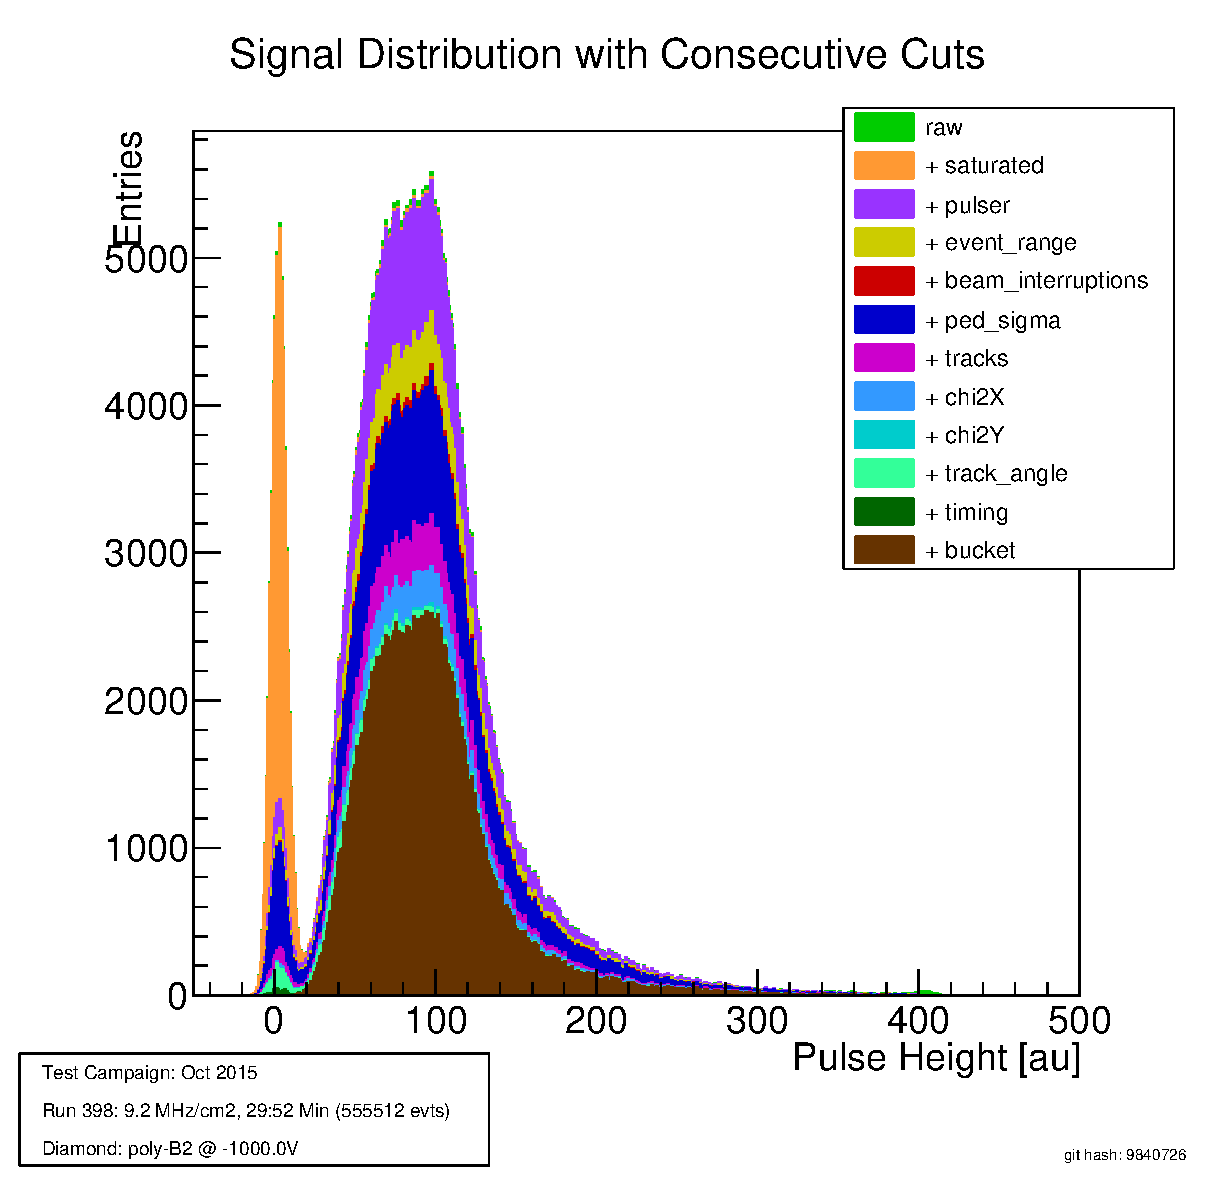
\includegraphics[angle=270, width=3.5cm]{consecutive398}\\
		\includegraphics[angle=270, width=3.5cm]{consecutive_logy398}
	\end{minipage}
\end{frame}
% new frame =======================
\begin{frame}
	\frametitle{Pulse Height Distribution}
	\begin{minipage}{4cm}
		\centering 
		\includegraphics[angle=270, width=3.0cm]{Landau}
	\end{minipage}
	\hspace*{2pt}
	\begin{minipage}{6.5cm}
		\centering
		\includegraphics[angle=270, width=6.0cm]{CutMeans}
	\end{minipage}
	\begin{minipage}{6cm}
		\begin{itemize}
			\item pedestal is completely gone after application of the cuts 
			\item wide Landau due to polycrystalline diamonds
			\item mean of the pulse height increases significantly due to cuts (pedestal goes away)
		\end{itemize}
	\end{minipage}
	\hspace*{2pt}
	\begin{minipage}{5cm}
		\centering
		\includegraphics[width=4cm]{Cuts}
	\end{minipage}
\end{frame}
% ============================
\subsection{Signal Map}
\begin{frame}
	\frametitle{Signal Map}
	\begin{center}
		\includegraphics[angle=270, width=5.5cm]{SignalMap}\\
	\end{center}
	\begin{itemize}
		\item different regions inside the diamond yield different average pulse heights
		\item does not change with rate or time
	\end{itemize}
\end{frame}
% END
% ====================================================================================
% BEGIN RESULTS
% ====================================================================================
\section{Results}
% ============================
\subsection{S129 (Element Six - single crystal)}
\begin{frame}
	\frametitle{$+$\SI{500}{V} August - unirradiated}
	\begin{minipage}{5.5cm}
		\centering
		\includegraphics[width=5cm]{PHS41}
	\end{minipage}
	\hspace*{2pt}
	\begin{minipage}{5.5cm}
		\centering
		\includegraphics[width=5cm]{PHSZ41}
	\end{minipage}\s
	\begin{itemize}
		\item amplifier issues during the last two runs
	\end{itemize}
\end{frame}
% new frame =======================
\begin{frame}
	\frametitle{$-$\SI{500}{V} October - unirradiated}
	\begin{minipage}{5.5cm}
		\centering
		\includegraphics[width=5cm]{PHS03}
	\end{minipage}
	\hspace*{2pt}
	\begin{minipage}{5.5cm}
		\centering
		\includegraphics[width=5cm]{PHSZ03}
	\end{minipage}
\end{frame}
% new frame =======================
\begin{frame}
	\frametitle{$+$\SI{500}{V} October - unirradiated}
	\begin{minipage}{5.5cm}
		\centering
		\includegraphics[width=5cm]{PHS05}
	\end{minipage}
	\hspace*{2pt}
	\begin{minipage}{5.5cm}
		\centering
		\includegraphics[width=5cm]{PHSZ05}
	\end{minipage}
\end{frame}
% ============================
\subsection{Poly-B2 (II-IV B2 - poly crystal)}
\begin{frame}
	\frametitle{$+$\SI{1000}{V} August - unirradiated}
	\begin{minipage}{5.5cm}
		\centering
		\includegraphics[width=5cm]{PH02}
	\end{minipage}
	\hspace*{2pt}
	\begin{minipage}{5.5cm}
		\centering
		\includegraphics[width=5cm]{PHZ02}
	\end{minipage}
\end{frame}
% new frame =======================
\begin{frame}
	\frametitle{$-$\SI{1000}{V} August - unirradiated}
	\begin{minipage}{5.5cm}
		\centering
		\includegraphics[width=5cm]{PH13}
	\end{minipage}
	\hspace*{2pt}
	\begin{minipage}{5.5cm}
		\centering
		\includegraphics[width=5cm]{PHZ13}
	\end{minipage}
\end{frame}
% new frame =======================
\begin{frame}
	\frametitle{$-$\SI{1000}{V} October - irradiated}
	\begin{minipage}{5.5cm}
		\centering
		\includegraphics[width=5cm]{PH81}
	\end{minipage}
	\hspace*{2pt}
	\begin{minipage}{5.5cm}
		\centering
		\includegraphics[width=5cm]{PHZ81}
	\end{minipage}
\end{frame}
% END 
% ====================================================================================
% CONCLUSION
% ====================================================================================
\section{Conclusion}
% ============================
\begin{frame}
	\frametitle{Conclusion}
	\begin{itemize}
		\setlength{\itemsep}{\fill}
		\item very good timing resolution with scintillator allows for precise integration and separation of the signal
		\item tested several diamond pad detectors with fluxes between \SI{1}{kHz/cm^{2}} and \SI{10}{MHz/cm^{2}}
		\item unirradiated single crystal shows almost no rate dependence
		\item most of the polies behave similarly
		\item some of the diamond pad detectors have only a very slight ($1-3$\%) rate dependence after irradiation
	\end{itemize}
\end{frame}
% ====================================================================================
% OUTLOOK
% ====================================================================================
\section{Outlook}
% ============================
\begin{frame}
	\frametitle{Outlook}
	\underline{\textbf{Event Synchroniser:}}
	\begin{itemize}
		\setlength{\itemsep}{\fill}
		\item fix unsynchronous runs (event misalignment)
		\item using pulser reference runs to check alignment
		\item writing program to detect and realign the runs
	\end{itemize}
	\vspace*{10pt}
	\underline{\textbf{Finish Analysis:}}
	\begin{itemize}
		\setlength{\itemsep}{\fill}
		\item vary and confirm cuts 
		\item create all final plots
		\item make a final presentation
	\end{itemize}
\end{frame}
% ============================
% DOCUMENT END
\end{document}

